\documentclass[ngerman]{scrbook}

\usepackage[utf8]{inputenc}
\usepackage[T1]{fontenc}
\usepackage{babel}
\usepackage{lmodern}
\usepackage{microtype}
\usepackage[colorlinks=true,linkcolor=blue]{hyperref}
\usepackage{makeidx}
\usepackage{enumitem}
\usepackage{graphicx}
\usepackage{subfigure}

\usepackage{amsmath}
\usepackage{amssymb}
\usepackage[version=4]{mhchem}
\usepackage[exponent-product=\cdot,per-mode=fraction]{siunitx}

\usepackage{tabularx}
\usepackage{tabulary}
\usepackage{booktabs}

\newcommand{\planck}{\mathtt{h}}
\newcommand{\sol}{\mathtt{c}}
\newcommand{\boltz}{\mathtt{k}}
\newcommand{\IN}{\mathbb{N}}
\renewcommand{\d}{\mathrm{d}}
\newcommand*{\e}[1]{e^{#1}}

\begin{document}
\title{B-Praktikum}
\author{Fabian Haneder}
\date{09.11.2016}
\maketitle[1]

\tableofcontents
\chapter{Optische Spektroskopie}
Im Jahr 1835 behauptete einst der französische Philosoph Auguste Comte, man würde nie etwas über die chemische Zusammensetzung der Sonne und der Sterne erfahren. Bereits 33 Jahre später entdeckten Sir Norman Loycker und Pierre Janssen ein bislang unbekanntes Element in der Sonne, das sie Helium nannten. Möglich war ihnen dies durch den Fortschritt der Spektroskopie, in die in diesem Versuch eingeführt werden soll.

Unter Spektroskopie versteht man physikalische Methoden, die dazu benutzt werden, elektromagnetische Strahlung und, gerade zu Anfang, vor allem sichtbares Licht nach einer bestimmten Eigenschaft wie der Wellenlänge zu zerlegen. Außer zur Untersuchung von Himmelskörpern können diese Methoden auch verwendet werden, um mittels Spektralanalyse oder Massenspektrometrie die chemische Zusammensetzung von unbekannten Proben sehr genau zu bestimmen. 

Aber nicht nur die Chemie, sondern auch die Physik hat durch Spektroskopie signifikante Fortschritte gemacht. So findet die Entwicklung der Atomphysik und  Quantenmechanik ihren Ausgangspunkt in der Beobachtung von Linienspektren verschiedener Atome und Moleküle, und auch Naturgesetze und -konstanten konnten durch spektroskopische Methoden untersucht werden.

In diesem Versuch soll, nachdem sich zunächst mit den zur Durchführung notwendigen Programmen und Analysemethoden vertraut gemacht wurde, das Sonnenspektrum ausgewertet werden. Zudem soll das für die Strahlung einer Glimmlampe verantwortliche Element identifiziert und schließlich die sogenannte additive Farbmischung untersucht werden.

\section{Vorbereitung}
\begin{enumerate}
	\item Wozu wird das Prinzip der Beugung in einem Spektrometer benötigt?
		\subitem Unterschiedliche Wellenlängen werden unterschiedlich stark gebeugt bzw. gebrochen, wodurch die Intensitätsmaxima unterschiedlicher Farben an unterschiedlichen Orten auftreten.
	\item Welche Vorteile hat ein Beugunsgitter im Vergleich zu einem Doppelspalt? Ändert sich die Lage der Maxima mit zunehmender Spaltanzahl?
		\subitem Bei einem Beugunsgitter lässt sich eine erheblich höhere Genauigkeit erzielen, da die Intensitätsmaxima deutlich schmaler und höher sind. So berechnet sich beispielsweiße die Fußpunktbreite wie folgt: $\Delta\beta=\lambda/N\cdot d$
		
		Hierbei ist $N$ die Spaltanzahl und $d$ der Spaltabstand. Mehr Spalten bedeutet also höhere Genauigkeit. Die Lage der Maxima ändert sich allerdings nicht.
	\item Beschreiben Sie das Spektrum eines Temperaturstrahlers und einer Gasentladungslampe.
		\subitem Temperaturstrahler strahlen stets ein kontinuierliches Spektrum ab, dessen Intensitätsmaximum bei Raumtemperatur im Normalfall außerhalb des sichtbaren Bereichs liegt. Wird die Temperatur erhöht, so verschiebt sich das Maximum in den sichtbaren Bereich und dort nach und nach von Rot über Gelb bis hin zu Blau.
		
		 Gasentladungslampen hingegen erzeugen ein Spektrum, bei dem die Maxima deutlich ausgeprägter auftreten, als beim kontinuierlichen Spektrum des Temperaturstrahlers. So kann zum Beispiel mit Natriumdampf-Lampen nahezu monochromatisches Licht erzeugt werden, lediglich die Bewegung der Natriumatome im heißen Dampf führt über den Dopplereffekt zur geringfügigen Verbreiterung der der Bandbreite des emittierten Lichts.
	\item Wie können mit Hilfe eines Spektrometers die chemischen Elemente der Erd- und Sonnenatmosphäre bestimmt werden? Wie können diese der jeweiligen Atmosphäre zugeordnet werden?
		\subitem Die Elemente der Erd- und Sonnenatmosphäre können durch einen Vergleich des Spektrums des Sonnenlichts mit bereits bekannten Emissionslinien der einzelnen Elemente bestimmt werden.
		Eine Zuordnung könnte etwa dadurch erfolgen, dass versucht wird, einen der Faktoren zu eliminieren, indem z.B. von einem Satelliten aufgefangenes Licht analysiert wird.
	\item Welche Temperatur (in Kelvin) besitzt die Sonnenoberfläche? Skizzieren Sie den Intensitätsverlauf eines schwarzen Körpers mit dieser Temperatur und kennzeichnen Sie die Strahldichte des sichtbaren Bereichs.
		\subitem \begin{figure}[!hbt]
			\centering
			\hypertarget{Abb1}{}
			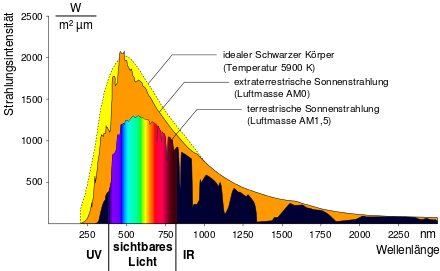
\includegraphics{sunspectrum}
			\caption{Intensitätsspektrum eines sonnenähnlichen Schwarzkörpers}
			\label{fig:Abb1}
		\end{figure}
		Hierzu benötigt man die Formeln für die spektrale Strahldichte und das Wien'sche Verschiebungsgesetz:
		\begin{align}
			L_{S,\lambda}(\lambda,T)&=\frac{\mathrm{c}_1}{\pi\lambda^{5}}\Big[\exp\Big(\frac{\mathrm{c}_2}{\lambda T}\Big)-1\Big]^{-1}\label{1}\\
			\lambda_{\mathrm{max}}T&=\SI{2.8978e-3}{\meter\kelvin}\label{2}
		\end{align}
		mit den Konstanten 
		\begin{align*}
			\mathrm{c}_1&=2\pi\planck\sol_0^2=\SI{3.7418e-16}{\watt\meter\squared}\\
			\mathrm{c}_2&=\planck\sol_0\boltz^{-1}=\SI{1.4388e-2}{\meter\kelvin}
		\end{align*}
		Die Sonnenoberfläche besitzt eine Temperatur von $T=\SI{5777}{\kelvin}$. Damit erreicht die Intensitätsverteilung ihr Maximum bei $\lambda_{\mathrm{max}}=\SI{5.016e-7}{\meter}$. Dies entspricht der Farbe Hellgrün. (Für Abbildung s. \hyperlink{Abb1}{hier})
		
	\item Wie hoch müsste die Temperatur eines schwarzen Körpers sein, damit das Intensitätsmaximum in der Mitte des sichbaren Bereichs liegt? Warum können solche Temperaturen nicht mit einem herkömmlichen Glühdraht erreicht werden?
		\subitem Nach dem Wien'schen Verschiebungsgesetz ergibt sich mit $\lambda_{\mathrm{avg}}=\SI{550}{\nano\meter}$:
		\begin{displaymath}
			T_{\mathrm{avg}}=\SI{5268}{\kelvin}
		\end{displaymath}
		Solche Temperaturen können mit herkömmlichen Glührähten aus Wolfram nicht erreicht werden, da Wolfram einen Schmelzpunkt von $T_{\mathrm{schmelz}}=\SI{3695}{\kelvin}$  aufweist.
	\item Wie kann die Temperatur eines Glühdrahtes relativ einfach (in guter Näherung) bestimmt werden, wenn der Verlauf des Spektrums der Strahlung bekannt ist? Wie kann diese bestimmt werden, wenn nur ein kleiner Ausschnitt des Verlaufs (z.B. nur der sichtbare Bereich) bekannt ist?
		\subitem Ist das gesamte Spektrum bekannt, so kann durch Ermittlung der Wellenlänge, bei der das Intensitätsmaximum auftritt, die Temperatur des Strahlers über das Wien'sche Verschiebungsgesetz recht einfach berechnen.
		Ist nur ein Teil des Spektrums bekannt, so kann aus dem Auftreten bestimmter Spektrallinien zumindest eine Mindesttemperatur extrapoliert werden, die nötig ist, um das Material des Glühdrahtes mit der entsprechenden Wellenlänge zum Leuchten zu bringen.
	\item Erklären Sie den Begriff der Farbtemperatur. Was sagt dieser Begriff über das Spektrum einer Glühlampe(Temperaturstrahler) und einer Energiesparlampe(Gasentladungslampe) aus?
		\subitem Unter Farbtemperatur versteht man die zu einer bestimmten Farbe gehörende Temperatur, die nötig ist, um einen schwarzen Körper unter festgelegter Helligkeit und  Beobachtungsbedingungen möglichst genau mit dieser Farbe zum Strahlen zu bringen. 
		
		Die Farbtemperatur von Energiesparlampen und anderen Gasentladungslampen ist im Normalfall bei ca. $\SI{4000}{\kelvin}-\SI{5000}{\kelvin}$ und damit höher, als bei Glühlampen (ca. $\SI{2600}{\kelvin}-\SI{3000}{\kelvin}$). Eine Ausnahme bilden hier lediglich Natriumdampflampen, deren Farbtemperatur etwa $\SI{2000}{\kelvin}$ beträgt. Damit ist im Allgemeinen eine höhere Temperatur nötig, um mit einem schwarzen Körper das Leuchten einer Energiesparlampe nachzuahmen, als das einer Glühbirne.
	\item Welcher proportionale Zusammenhang besteht zwischen spezifischer Ausstrahlung und Temperatur eines schwarzen Körpers? Welches Gesetz beschreibt diesen Zusammenhang?
		\subitem Wie oben bereits beschrieben, hängen die spezifische Ausstrahlung und Temperatur eines schwarzen Körpers über das Wien'sche Gesetz \eqref{2} zusammen.
	\item Wie kann mit Hilfe eines Spektrometers auf die chemischen Inhaltsstoffe von Gasentladungslampen geschlossen werden?
		\subitem Die Spektra von Gasentladungslampen haben meist sehr ausgeprägte Maxima, man spricht auch von Linienspektra. Vergleicht man die Wellenlängen dieser Peaks mit den Emissionsspektra von bekannten Stoffen, so lässt sich auf die chemische Zusammensetzung des jeweiligen Leuchtstoffs schließen.
\end{enumerate}
\section{Durchführung}
\subsection{Allgemeine Hinweise}
Zum Wechseln der Lampen (230 Volt!)
\begin{itemize}
	\item Lampe vor Wechseln ausschalten und abkühlen lassen
	\item Nicht die Kontakte in der Fassung berühren
\end{itemize}
Zum Umgang mit dem Lichtwellenleiter
\begin{itemize}
	\item Zu starke Krümmung vermeiden ($r\geq\SI{15}{\centi\meter}$)
	\item Unnötige Verspannungen des Knickschutzes vermeiden
	\item Berührungen mit dem Lichtwellenleitereingang vermeiden, diesen nach Versuchsende verschließen
	\item Abstand zwischen Lampe und Leiter min. $\SI{15}{\centi\meter}$
\end{itemize}
Zur Versuchsdurchführung
\begin{itemize}
	\item Auf möglichst wenig Umgebungslicht achten
	\item Dunkel- und Referenzspektrum aktuell halten
	\item Richtige Parameter beim Speichern angeben
	\item Diagramme mit allen relevanten Angaben beschriften
\end{itemize}
\subsection{Einführende Versuche}
\subsubsection{Einführung in SpectraWiz}
Öffnen Sie SpectraWiz und wechseln Sie ggf. in den Scope-Modus. Setze die Parameter folgendermaßen:
\begin{displaymath}
	\mathrm{\textsc{SCOPE -> ... Time: 100 ms, Avg:1, Sm:0, Sg:0, Tc:off, Xt:3, Ch:1}}
\end{displaymath}
Richten Sie den Lichtwellenleiter auf die Glühlampe aus und fixieren Sie ihn mithilfe des Stativmaterials. Speichern Sie bei abgeschalteter Lampe das Dunkelspektrum.
\begin{itemize}[label=$\blacktriangleright$]
	\item Wozu wird das Dunkelspektrum benötigt?
\end{itemize}
Justieren Sie den Lichtwellenleiter so, dass das Maximum des Graphen im obersten Viertel der Skala liegt.
\begin{itemize}[label=$\blacktriangleright$]
	\item Wie wirkt sich eine Änderung der Parameter "\textsc{Detector integration time}" und "\textsc{Number of scans to average}" auf die Anzeige aus?
\end{itemize}
Nehmen Sie das Spektrum der Glühlampe auf und speichern Sie es ab. 
\begin{itemize}[label=$\blacktriangleright$]
	\item Begründen Sie, warum die angezeigte Intensitätsverteilung nicht der tatsächlichen Verteilung des Glühlampenspektrums entsprechen kann.
\end{itemize}
\subsubsection{Aufnahme von Transmissionsspektren}
Nehmen Sie das Glülammpenspektrum als Referenzspektrum auf und wechseln Sie in den Transmissionsmodus
\begin{itemize}[label=$\blacktriangleright$]
	\item Wozu wird das Referenzsprektrum benötigt?
	\item Woran lässt ich im Transmissionsmodus erkennen, ob das Referenzspektrum und das Dunkelspektrum richtig eingestellt, bzw. ob die beiden noch aktuell sind?
	\item Warum ist im Wellenlängenbereich unterhalb von ca. $\SI{350}{\nano\meter}$ keine sinnvolle Transmissionsmessung möglich?
\end{itemize}
Halten Sie farbige Brillengläser in den Strahlengang.
\begin{itemize}[label=$\blacktriangleright$]
	\item Beschreiben Sie qualitativ Ihre Beobachtungen bzgl. der Farbe und des dazugehörigen Transmissionsspektrums.
\end{itemize}
Nehmen Sie die Transmissionsspektra zweier einzelner Gläser und dasd Spektrum der Kombination auf und speichern Sie sie ab. Stellen Sie die Spektra in QtiPlot in einem Diagramm dar und drucken Sie dieses aus.
\begin{itemize}[label=$\blacktriangleright$]
	\item Welcher mathematische Zusammenhang gilt für die einzelnen eben erwähnten Transmissionsgrade?
\end{itemize}
(\#) Ermitteln Sie in QtiPlot rechnerisch das Transmissionsspektrum der Filterkombination. Stellen Sie dieses zusammen mit den anderen Spektren in einem Diagramm dar.
\subsubsection{Aufnahme von Emissionsspektren}
Nehmen Sie im Scope-Modus das Spektrum einer Energiesparlampe auf und speichern Sie dieses ab.
\begin{itemize}[label=$\blacktriangleright$]
	\item Beschreiben Sie qualitativ die Unterschiede zum Spektrum einer Glühlampe.
\end{itemize}
Nehmen Sie die Spektren der LEDs (rot, grün, blau) auf.
\begin{itemize}[label=$\blacktriangleright$]
	\item Notieren Sie sich zu den einzelnen Farben der LEDs die Wellenlängenwerte der Maxima, welche Sie in SpectraWiz bestimmen können.
	\item Lässt sich durch diese Werte auf den jeweiligen Farbeindruck schließen? Begründen Sie Ihre Aussage.
\end{itemize}
\subsubsection{Bestimmung der Farbtemperatur einer Glühlampe}
Öffnen Sie in QtiPlot die Umrechnungstabelle und importieren Sie das Glühlampenspektrum. Führen Sie die für die Umrechnung erforderlichen Schritte aus und stellen Sie das angepasste Spektrum dar.
\begin{itemize}[label=$\blacktriangleright$]
	\item Warum müssen zur Bestimmung der Farbtemperatur die Messdaten umgerechnet werden?
	\item Begründen Sie qualitativ, wie und wie stark sich die angelegte Wechselspannung ($f=\SI{50}{\hertz}$) im Vergleich zu einer entsprechenden Gleichspannung auf die Farbtemperatur auswirkt.
\end{itemize}
Erstellen Sie mittels des Fit-Assistenten eine geeignete Kurve für den Wellenlängenbereich von ca. 1-2000nm. Drucken Sie das Diagramm, in dem die ermittelte Temperatur ersichtlich ist, aus.
\begin{itemize}[label=$\blacktriangleright$]
	\item Beschreiben Sie mit Hilfe des Graphen, warum eine Glühlampe als Beleuchtungsmedium nicht effizient ist.
	\item Bestimmen Sie mit Hilfe des Wien'schen Verschiebungsgesetzes die Lage des Maximums des angezeigten Schwarzkörperspektrums.
\end{itemize}
\subsection{Erzeugung verschiedener Farbtemperaturen mit einem Glühlämpchen}
Nehmen Sie drei verschiedene Spektra durch Änderung der Spannung (max. 10 Volt!) zu den subjektiv empfundenen Intensitäten "schwach", "mittel" und "stark" auf.

Ermitteln Sie in QtiPlot die Farbtemperaturen und speichern Sie die Diagramme ab.
\begin{itemize}[label=$\blacktriangleright$]
	\item Begründen Sie qualitativ, wie und warum sich die angelegte elektrische Spannung auf das aufgenommene Spektrum auswirkt.
\end{itemize}
\subsection{Auswertung des Sonnenspektrums}
\subsubsection{Aufnahme des Sonnenspektrums}
Richten Sie den Lichtwellenleiter so aus, dass Sie das Sonnenspektrum aufnehmen können (Aufnahme des Streulichts genügt). Speichern Sie bei aktuell gehaltenem Dunkelspektrum die Intensitätsverteilung ab.
\subsubsection{Bestimmung der Oberflächentemperatur der Sonne}
Rechnen Sie die Messdaten in QtiPlot um und stellen Sie sie graphisch dar. Erstellen Sie eine Fit-Kurve* und drucken Sie das Diagramm mit Angabe der ermittelten Oberflächentemperatur aus.

*Für den Fall, dass keine geeignete Kurve ermittelt werden kann, stellen Sie den Verlauf eines Schwarzkörperspektrums für $T=\SI{6000}{\kelvin}$ dar.
\begin{itemize}[label=$\blacktriangleright$]
	\item Begründen Sie kurz einige bei dieser Auswertung vorliegende Fehlerquellen.
\end{itemize}
\subsubsection{Bestimmung der wichtigsten Fraunhofer'schen Linien}
Stellen Sie das Sonnenspektrum in einem neuen Diagramm dar. Drucken Sie den Graphen aus. Bestimmen Sie mit Hilfe des "Datenlesers" die Wellenlängen der "Einbrüche" im Spektrum, welche den jeweiligen Fraunhofer'schen Linien entsprechen (vgl. Tabelle).		
\begin{enumerate}[label=$\blacktriangleright$]
	\item Kennzeichnen Sie die Lage diser Linien im Diagramm.
	\item Notieren Sie die gemessenen Wellenlängenwerte und bestimmen Sie die Differenz zu den Tabellenwerten.
	\item Wie lässt sich diese Differenz erklären?
\end{enumerate}
\begin{table}
	\caption{Wichtige Fraunhofer'sche Linien} \label{tab: flines}
	\centering
	\begin{tabular}{>{\bfseries}lll}
		\toprule[2pt]	Symbol&$\lambda$[nm]&Element\\
		\midrule[2pt]	A&$760.8$&\ce{O}\\
		\midrule		B&$686.7$&\ce{O}\\
		\midrule		C&$656.3$&\ce{H}\\
		\midrule		D\textsubscript{1}&$589.6$&\ce{Na}\\
		\midrule		D\textsubscript{2}&$589.0$&\ce{Na}\\
		\midrule		E&$527.0$&\ce{Fe}\\
		\midrule		F&$486.1$&\ce{H}\\
		\midrule		G&$430.8$&\ce{Fe}\\
		\midrule		H&$396.8$&\ce{Ca}\\
		\midrule		K&$393.4$&\ce{Ca}\\
		\bottomrule[2pt]
	\end{tabular}
\end{table}
\subsection{Bestimmung chemischer Elemente}
Stellen Sie das Spektrum einer Glimmlampe im Scope-Modus dar. Dieses erhalten Sie durch Aufnahme der Schalterbeleuchtung einer Steckdosenleiste. Justieren Sie hierzu den Lichtwellenleiter senkrecht über dem Schalter in wenigen Zentimetern Abstand.
\begin{enumerate}[label=$\blacktriangleright$]
	\item Erläutern Sie qualitativ, ob und wie der transparente gefärbte Kunststoff des Schalters die Aufnahme des Spektrums beeinflusst.
	\item Warum ist für diesen Versuchsteil keine Umrechnung der Daten in QtiPlot notwendig?
\end{enumerate}
Werten Sie das abzuspeichernde Spektrum in QtiPlot aus. Bestimmen Sie mittels ausliegender Messdaten bekannter Stoffe das für die Strahlung verantwortliche Element in der Lampe.

Importieren Sie zusätzlich die Messdaten des passenden Vergleichsspektrums und stellen Sie dieses im gleichen Diagramm dar.
\begin{enumerate}[label=$\blacktriangleright$]
	\item Welchen Vorteil hat dieses Verfahren gegenüber der Auswertung mit Hilfe von Tabellenwerten?
\end{enumerate}
Beschriften Sie markante Peaks mit zugehörigen Wellenlängen und drucken Sie das Diagramm aus.

(\#)Belegen Sie graphisch, dass in einer Energiesparlampe Anteile von Quecksilber vorhanden sind. Drucken Sie anschließend Ihre Ergebnisse mit geeigneter Beschriftung aus.
\subsection{Additive Farbmischung}
Betrachten Sie im Scope-Modus das Spektrum der farbwechselnden LED-Lampe und beantworten Sie folgende Fragen:
\begin{enumerate}[label=$\blacktriangleright$]
	\item Wie viele verschiedenfarbige LEDs werden in dieser Lampe eingesetzt?
	\item Welche (Peak-)Wellenlängen und Farben haben diese LEDs?
	\item Nennen Sie zusätzlich ein Beispiel, an dem ersichtlich wird, warum aufgrund eines Farbeindrucks nicht auf die zugrundeliegenden Wellenlängen geschlossen werden kann.
\end{enumerate}
Veranschaulichen Sie sich die additive Farbmischung mittels LEDs, deren Helligkeit einzeln verändert werden kann. Versuchen Sie, Mischfarben zu erzeugen. Verwenden Sie die Lampe als Streumedium. Richten Sie die LEDs auf eine weiße Fläche und erzeugen Sie Schatten in verschiedenen Farben.
\begin{enumerate}[label=$\blacktriangleright$]
	\item Erklären Sie das Zustandekommen dieser bunten Schatten.
\end{enumerate}
\chapter{Lichtbeugung an Spalt und Gitter}
In diesem Versuch soll das auch in der Spektroskopie Anwendung findende Prinzip der Beugung elektromagnetischer Wellen an einem oder mehreren Spalten genauer untersucht werden. Hierzu wird mit monochromatischem Licht gearbeitet, sodass aus der Theorie bekannte Beugungsgesetze, die in der Regel von der Wellenlänge des benutzten Lichts abhängen, möglichst gut überprüft werden können. Hier sollen zunächst die Zusammenhänge für den Einzelspalt angegeben werden:
\begin{align*}
	\sin(\phi_{k,min})&=\frac{\lambda}{b}\cdot k\\
	\sin(\phi_{k,max})&=\frac{\lambda}{b}\cdot\Big(k+\frac{1}{2}\Big)\\
	\phi_{0,max}&=0
\end{align*}
Hierbei ist $\lambda$ die Wellenlänge, $b$ die Spaltbreite und $k\in\IN$ die Beugungsordnung.

Fügt man einen zweiten Spalt (mit gleicher Spaltbreite) im Abstand $d$ hinzu, so erhält man zusätzlich zu den Beugungsextrema Interferenzeffekte, die ebenfalls zu Extrema führen, die sich folgendermaßen berechnen:
\begin{align*}
	\sin(\Psi_{m,min})&=\frac{\lambda}{d}\Big(m+\frac{1}{2}\Big)\\
	\sin(\Psi_{m,max})&=\frac{\lambda}{d}\cdot m
\end{align*}
Hierbei ist $m\in\IN_{0}$

Erweitert man diesen Aufbau erneut zu einem Gitter mit $N$ gleich breiten Spalten im gleichen Abstand, so ergibt sich eine etwas unhandlichere Beziehung für die Intensität des Lichtes in Richtung $\phi$:
\begin{displaymath}
	I(\phi)=\Bigg(\frac{\sin\Big(\frac{\pi b}{\lambda}\sin\phi\Big)}{\frac{\pi b}{\lambda}\sin\phi}\Bigg)^2\Bigg(\frac{\sin\Big(\frac{N\pi b}{\lambda}\sin\phi\Big)}{\sin\Big(\frac{\pi b}{\lambda}\sin\phi\Big)}\Bigg)^2
\end{displaymath}
\section{Vorbereitung}
\begin{enumerate}
	\item Nehmen Sie an, die Beugung findet nicht in Luft $(n\approx1)$, sondern in Wasser statt $(n>1)$. Wie ändert sich das Beugungsbild?
		\subitem Da Wasser ein optisch dichteres Medium ist, als Luft, wird die Wellenlänge verringert:
		\begin{displaymath}
			\lambda'=\frac{c'}{\nu}=\frac{c}{\nu}\cdot\frac{1}{n}=\frac{\lambda_0}{n}
		\end{displaymath}
		Dies bedeutet, da $\phi\in[0,\frac{\pi}{2}]$, dass die Winkel, unter denen die Extrema auftreten, kleiner werden.
	\item Es werde zuerst das Beugungsbild eines Doppelspaltes fotografisch aufgenommen; auf einem gleichartigen Film werden dann nacheinander die Beugungsfiguren beider Einzelspalte auf demselben Film aufgenommen. Insgesamt werden beide Filme gleich lange belichtet. Vergleichen Sie die Beugungsbilder miteinander. Erklären Sie Gleichheit oder Ungleichheit.
		\subitem Die Beugungsbilder unterscheiden sich, da die physikalischen Vorgänge nicht vollkommen gleich sind. Werden die Bilder der Einzelspalte aufgenommen, so addieren sich schlichtweg die Intensitäten:
		\begin{displaymath}
			I=I_1+I_2
		\end{displaymath}
		Beim Doppelspalt werden hingegen die Felder addiert, nicht die Intensität. Diese ist proportional zum Feldquadrat:
		\begin{displaymath}
			I\propto\vec{E}^2=(\vec{E}_1+\vec{E}_2)^2=\underbrace{\vec{E}_1^2}_{\propto I_1}+\underbrace{\vec{E}_2^2}_{\propto I_2}+2\vec{E}_1\cdot\vec{E}_2
		\end{displaymath}
		Die Gesamtintensität ist beim Doppelspalt daher nicht identisch mit der zweier Einzelspalten.
	\item Nehmen Sie an, bei einem Doppelspalt werden die beiden Spalte jeweils von verschiedenen Lasern beleuchtet. Wie würde sich das Beugungsbild gegenüber dem üblichen Experiment ändern?
		\subitem Wenn die Laser die gleiche Wellenlänge abstrahlen, ergibt sich das (bis auf durch eventuelle Phasenunterschiede hervorgerufene Schwebungen) gleiche Beugungsbild, wie bei der normalen Beugung des Lichtes einer Lichtquelle an einem Doppelspalt. Weisen die Laser unterschiedlicher Wellenlängen auf, so wirkt jeder Spalt als Einzelspalt für die jeweilige Lichtquelle.
	\item Nehmen Sie an, ein Laserstrahl wird durch Spiegel aufgespalten und die beiden Strahlen beleuchten je einen Spalt. Besteht ein Unterschied zu dem vorher geschilderten Fall? Wenn ja, erklären Sie, weshalb.
		\subitem Wird der Laser aufgespalten, so können Phasenunterschiede zwischen den Teilstrahlen entstehen, was wie im obigen Fall zu Schwebungen führen kann. Ansonsten ergibt sich das gleiche Bild
	\item Wie ändert sich das Beugungsbild eines Spaltes, wenn dieser statt mit einem Laser mit Licht einer Hg-Dampflampe beleuchtet wird?
		\subitem Das Licht einer Quecksilberlampe ist nicht monochromatisch, sondern weißt im sichtbaren Bereich gleich 6 unterschiedliche Emissionslinien auf, die daher auch unterschiedlich gegbeugt werden. Daher kann man im Beugungsbild Extrema unterschiedlicher Wellenlängen an unterschiedlichen Orten beobachten.
	\item Was unterscheidet Fraunhofer- und Fresnel-Beugung?
		\subitem Die Fraunhofer-Näherung der Lichtbeugung ist eine Fernfeldnäherung, die Fresnel-Näherung hingegen eine Nahfeldnäherung. Dies hat zur Folge, dass beispielsweiße das Beugungsintegral unter der Fraunhofer'schen Betrachtung recht einfach zu lösen ist, da es lediglich die Form einer Fourier-Transformierten hat. In Fresnel-Näherung hingegen ist dies nicht der Fall, und das Beugungsintegral ist im Allgemeinen nur numerisch zu lösen.
	\item Leiten Sie für den Einfachspalt die Formel $I(\phi)=I_0\Big(\frac{\sin\frac{\theta}{2}}{\frac{\theta}{2}}\Big)^2$ mit $\theta=\frac{2\pi}{\lambda}\cdot b\cdot\sin\phi$ und $I_0=I(\phi=0)$ für die Intensitätsverteilung in Abhängigkeit vom Beugungswinkel $\phi$ ab.
	
	Berechnen Sie das Intensitätsverhältnis $I(\phi_{k,max})/I(\phi=0)$ für die erste $(k=1)$ und zweite $(k=2)$ Beugungsordnung.
		\subitem Das elektrische Feld am Schirm erhält man zunächst durch Fouriertransformation:
		\begin{multline*}
			E(k_x,k_y)=E_0\int_{-\infty}^{\infty}\d x\int_{-\infty}^{\infty}\d y\Sigma_{Spalt}\e{-\imath k_xx}\e{-\imath k_yy}=E_0\delta(k_y)\cdot\int_{-\frac{b}{2}}^{\frac{b}{2}}\e{-\imath k_xx}\d x\\
			=E_0\delta(k_y)\frac{\e{-\imath k_x\frac{b}{2}}-\e{\imath k_x\frac{b}{2}}}{k_x}=E_0\cdot b\cdot\delta(k_y)\frac{\sin(k_x\frac{b}{2})}{k_x\frac{b}{2}}\\
			\Rightarrow I(k_x)=E(k_x)^2=I_0\frac{\sin^2(k_x\frac{b}{2})}{(k_x\frac{b}{2})^2}
		\end{multline*}
		Mit $k_x=\sin\phi\cdot\frac{2\pi}{\lambda}$ und $\theta=\frac{2\pi}{\lambda}\cdot b\cdot\sin\phi$ folgt:
		\begin{displaymath}
			I(\phi)=I_0\frac{\sin^2(\frac{\pi\cdot b}{\lambda}\sin\phi)}{(\frac{\pi\cdot b}{\lambda}\sin\phi)^2}=I_0\frac{\sin^2(\frac{\theta}{2})}{(\frac{\theta}{2})^2}
		\end{displaymath}
		Für die $k$-te Beugungsordnung gilt:
		\begin{displaymath}
			\sin(\phi_{k,max})=\frac{\lambda}{b}\Big(k+\frac{1}{2}\Big)
		\end{displaymath}
		Für die zu berechnenden Intensitätsverhältnisse erhält man somit:
		\begin{align*}
			\frac{I(\phi_{k,max})}{I_0}&=\frac{I_0\frac{\sin^2(\frac{\pi b}{\lambda}\sin\phi)}{\frac{\pi b}{\lambda}\sin\phi}}{I_0}=\frac{\sin^2(\frac{\pi b}{\lambda}\cdot\frac{\lambda}{b}(k+\frac{1}{2}))}{(\frac{\pi b}{\lambda}\cdot\frac{\lambda}{b}(k+\frac{1}{2}))^2}=\frac{\sin^2(\pi(k+\frac{1}{2}))}{(\pi(k+\frac{1}{2}))^2}\\
			\frac{I(\phi_{1,max})}{I_0}&=\frac{\sin^{2}(\pi(1+\frac{1}{2}))}{(\pi(1+\frac{1}{2}))^2}=\frac{4}{9\pi^2}\approx 0.045\\
			\frac{I(\phi_{2,max})}{I_0}&=\frac{sin^2(\pi(2+\frac{1}{2}))}{(\pi(2+\frac{1}{2}))^2}=\frac{4}{25\pi^2}\approx 0.016
		\end{align*}
	\item Verifizieren Sie für den Doppelspalt den Ausdruck $I(\phi)=4\cdot I_0\cdot(\frac{\sin\frac{\theta}{2}}{\frac{\theta}{2}})^2\cdot\cos^2\frac{\delta}{2}$ mit $\theta=\frac{2\pi}{\lambda}\cdot b\cdot\sin\phi$ und $\delta=\frac{2\pi}{\lambda}\cdot d\sin\phi$ und $I_0$ aus Frage 7. Begründen Sie anschaulich das Auftreten des Faktors 4 und berechnen Sie die Intensität des ersten Nebenmaximums $m=1$ relativ zum nullten in Abhängigkeit von Spaltbreite $b$ und Spaltabstand $d$. Für welches Verhältnis $d/b$ fällt das fünfte Nebenmaximum mit dem ersten Haupt-Minimum zusammen?
		\subitem Wie bereits oben beschrieben, werden beim Doppelspalt die Felder der hier um $\pm\frac{d}{2}$ verschobenen Einzelspalte überlagert. Bei der Fouriertransformation taucht nun ein zusätzlicher Phasenterm auf:
		\begin{displaymath}
			E_{Spalt,\nu}=E_{Spalt}\cdot\e{-\imath k_xx\frac{d}{2}}
		\end{displaymath}
		Für den Doppelspalt ergibt sich somit:
		\begin{displaymath}
			E_{DS}=E_{Spalt}\Big(\e{-\imath k_xx\frac{d}{2}}+\e{\imath k_xx\frac{d}{2}}\Big)=2\cdot E_0\frac{\sin(\frac{\theta}{2})}{\frac{\theta}{2}}\cdot\cos\Big(\frac{\pi\cdot d}{\lambda}\sin\phi\Big)
		\end{displaymath}
		Mit dem angegebenen $\delta$ berechnet sich die Intensität durch Quadrieren der Feldstärke zu
		\begin{displaymath}
			I_{DS}=4\cdot I_0\cdot\Big(\frac{\sin\frac{\theta}{2}}{\frac{\theta}{2}}\Big)^2\cdot\cos^2\Big(\frac{\delta}{2}\Big)
		\end{displaymath}
		Der Faktor $4$ taucht also auf, weil zunächst zwei Felder gleichre Amplitude addiert werden, und das resultierende Feld $2E_0$ anschließend quadriert wird.
		
		Für das Nebenmaximum $m$-ter Ordnung gilt:
		\begin{displaymath}
			\sin\Psi=\frac{\lambda}{d}\cdot m
		\end{displaymath}
		Damit erhält man für das Verhältnis der Intensitäten des ersten zum nullten Nebenmaximum analog zu Aufgabe 7:
		\begin{displaymath}
			\frac{I(\Psi_{1,max})}{I_0}=\Bigg(\frac{\sin(\frac{\pi b}{d})}{\frac{\pi b}{d}}\Bigg)^2
		\end{displaymath}
		Damit das 5. Nebenmaximum mit dem erten Hauptminimum zusammenfällt, muss gelten:
		\begin{displaymath}
			\frac{\lambda}{d}\cdot 5=\frac{\lambda}{b}\Rightarrow\frac{d}{b}=5
		\end{displaymath}
\end{enumerate}
\section{Durchführung}
\subsection{Beugungsbild des Einfachspaltes}
\begin{enumerate}[label=\alph*)]
	\item Nehmen Sie die Intensitätskurve der Beugungsfigur eines Einfachspaltes auf.
	\item Berechnen Sie aus Ihren Messdaten die Spaltbreite. Finden Sie eine andere optische Messmethode zur Bestimmung der Spaltbreite und vergleichen Sie beide Ergebnisse miteinander.
	\item Werten Sie auch die Intensitätsverhältnisse aus und vergleichen Sie die Ergebnisse mit der Beugungstheorie.
\end{enumerate}
\subsection{Beugungsbild des Doppelspaltes}
\begin{enumerate}[label=\alph*)]
	\item Wiederholen Sie die obige Messung für einen Doppelspalt. Was fällt am Beugungsbild, was an der Intensitätskurve des Beugungsbildes auf?
	\item Erklären Sie die Intensitätskurven mit der Beugungstheorie.
	\item Kontrollieren Sie das Verhältnis der Intensitäten von 0. und 1. Maximum 2. Klasse. Vergleichen Sie mit der Theorie. Überlegen Sie alle Fehlermöglichkeiten, um Abweichungen von Experiment und Theorie zu erklären.
\end{enumerate}
\subsection{Beugungsbild eines optischen Gitters}
\begin{enumerate}[label=\alph*)]
	\item Nehmen Sie die Intensitätskurve der Beugungsfigur eines optischen Gitters auf.
	\item Vergleichen Sie die Kurve für den N-fachen Spalt mit der Kurve des Doppelspalts.
	\item Berechnen Sie aus den Messdaten den mittleren Spaltabstand (Gitterkonstante)
	\item Versuchen Sie, den Einfluss des Einzelspaltes auf das Beugungsbild zu sehen.
\end{enumerate}
\chapter{Optische Geräte}
Bei diesem Versuch soll selbständig mit einfachen, aber grundsätzlich wichtigen optischen Geräten experimentiert werden. Im Vordergrund steht hier also das eigene Beobachten. Die quantitative Auswertung beruht auf den Gesetzten der geometrischen Optik. Konkret lässt sich dies an folgenden Aufgaben festmachen:
\begin{itemize}
 \item  Theoretische Überlegungen und Berechnungen experimentell überprüfen
 \item Grundgesetze der geometrischen Optik durch Anwenden besser verstehen
 \item  Probleme der geometrischen Optik praktisch lösen
 \item  Versuchsaufbauten justieren und optimieren
 \item Wichtige optische Geräte und Instrumente (Lupe, Fernrohre, Projektionsapparat, Mikroskop)
 in offener Versuchsanordnung nachbauen
\end{itemize}
Es wird mit folgenden Geräten experimentiert:
\begin{itemize}
 \item Lupe: Konvexlinse, die ein vergrößertes virtuelles Bild des Gegenstandes erzeugt, der sich innerhalb der Brennweite befindet
 \item Astronomisches Fernrohr: (auch Keplersches Fernrhr genannt) besteht aus zwei Sammellinsen
 \item Terrestrisches Fernrohr: besteht aus drei Linsen, wobei die Zwischenlinse der Bildumkehr dient
 \item Das holländische Fernrohr (Galileiisches Fernroht): aufgebaut aus Sammel- und Zerstreuungslinse
 \item Diaprojektor: aufgebaut aus Lampe, Kondensator, Objektiv und Schirm
 \item Erzeugung eines vergrößerten, auf dem Kopf stehenden, seitengedrehten Bild
 \item zwei Strahlengänge: beleuchtend und abbildend
 \item Mikroskop: Entwerfung eines reelen Zwischenbildes in vergößertem Maßstab, welches mit einer Lupe beobachtet wird
\end{itemize}
\newpage
\section{Fragen zur Vorbereitung}
1. Wie lautet die Abbildungsgleichung für dünne Sammel- und Zerstreuungslinsen? Welche Näherungen werden bei der Herleitung gemacht? Was ist die Hauptebene einer Linse?\\
Abbildungsgleichung für dünne Linsen:   $\frac{1}{b}+\frac{1}{g}=\frac{1}{f}=(n-1)\left(\frac{1}{r_1-r_2}\right)$ falls $d \ll r_1, r_2$\\
g= Gegenstandsweite \\
b= Bildweite\\
f= Brennweite\\ \\
Hauptebene: zwei in einem Abbildungssystem definierte Ebenen, in denen vereinfacht die Brechungen der Lichtstraheln angenommen werdenm im Raum zwischen den Hauptebenen werden die Lichtstrahlen parallel zur optischen Achse verlaufend gedacht\\
2. Wodurch werden die Bildhelligkeit und das Gesichtsfeld beeinflusst bzw. begrenzt?\\
Gesichtsfeld = allle zentralen peripheren Gegenstände und Punkte des Außenraums, die bei ruhiger, gerader Kopfhaltung und geradeaus gerichteten, bewegungslosem Blick wahrgenommen werden können, auch ohne sie direkt zu fixieren\\
Umfang des Gesichtsfeldes ist abhängig von der Pupillenweite und der Lage des Auges zu den Nachbarorganen (Nase, Augenlid). Bei teif in der Augenhöhle sitzenden Augen ist das Gesichtsfeld kleiner. An der Innenseite ist die größte Ausdehnung, an der Innenseite die kleinste. Die Farbenempfindlichkeit ist nicht an allen Stellen gleich - die äußerste Peripherie des Gesichtsfeldes ist die "farbenlose Zone", nach der Mitte zu folgt des Gesichtsfeld von blau, gelb, rot und grün. \\
Bildhelligkeit = Beleuchtungsstärke in der Bildebene eines abbildenden Systems oder Grauwert (digitales Bild)
Bild wird heller, je größer der Linsendurchmesser ist, d.h. je mehr von der Strahlungsenergie einfangen werden kann. \\\\
3. Leiten Sie die Formeln für die Vergrößerung von Lupe, den Fernrohren und dem Mikroskop
her. Berücksichtigen Sie beim Fernrohr insbesondere die großen Gegenstandsweiten.\\
Allgemein gilt:
\begin{align*}
%\begin{center}
V=\frac{\text{Sehwinkel mit Instrument}}{\text{Sehwinkel ohne Instrument}}=
\frac{\text{Sehwinkel mit Instrument}}{\text{Sehwinkel im Abstand $S_0$}}=
\frac{\epsilon}{\epsilon_0} \\
V_{Lupe}=\frac{\epsilon}{\epsilon_0}=\frac{G}{f_l}*\frac{S_0}{G}=\frac{S_0}{f_l} \\
V_{Mikroskop}=V_{Objektiv} \cdot V_{Okular}=\frac{l \cdot S_0}{f_{Obj} \cdot f_{Oku}}\\ (l=Tubulänge)\\
V_{Fernrohr}= V_{Objektiv} \cdot V_{Okular}= \frac{\frac{B}{S_0}}{\frac{G}{g}}=\frac{f_{Objekiv}}{f_{Okular}}\\
V_{Holländisches Fernrohr}=\frac{f_{Objektiv}}{|f_{Okular}|}\\
%\end{center}
\end{align*}
\\4. In welche Entfernungsbereiche - bezogen auf die Brennweite der Lupe - können der zu betrachtende Gegenstand und das Auge gebracht werden?\\
Bei einer Lupe beträgt der ideale Abstand zum Auge 25 cm, wenn der Gegenstand im Brennpunkt liegt. Liegt der Gegenstand zwischen Brennpunkt und Linse, ist das Auge angespannt, man muss das Auge auch näher an die Linse bringen. Falls sich der Gegenstand hinter der Brennweite befindet, kann er nicht mehr vergrößert gesehen werden.\\
\\5. Warum benutzt man in der Praxis meist Prismenfernrohre? Zeichnen Sie den Strahlengang!\\
\begin{figure}[h]
 \centering
 \subfigure[Strahlengang bei Umkehrprismen] {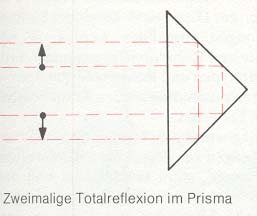
\includegraphics[width=0.49\textwidth]{prismenumkehr1}}
 % \caption{Gesichtsfeldblende und Umkehrprismen}
 \subfigure[Bildumkehr]{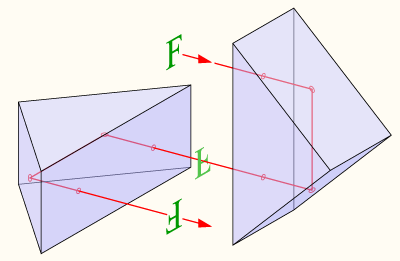
\includegraphics[width=0.49\textwidth]{prismenumkehr2}}
\end{figure}
Das Prismenfernrohr besteht wie das astronomische Fernrohr aus Obetiv und Okular. Das astronomische Fernrohr ergibt aber ein kopfstehtendes Bild. Zur Umkehrung dieses Bildes werden Prismen benutzt. Da bei dem kopfstehenden Bild auch links und rechts vertauscht werden, muss der Strahlengang noch ein zweites Prisma durchlaufen, damit auch die Seitenrichtigkeit wiederhergestellt ist. Diese Prismenanordnung bringt gegenüber dem terrestrischen Fernrohr durch den 3fach nebeneinanderglegten Strahlengang eine wesentlich verkürzte Baulänge. Der gegenüber dem Augenabstand vergrößerte Objektivabstand ist für das räumliche Sehen von Vorteil. \\ \\
6. Erläutern Sie anhand einiger einfacher optischer Abbildungsanordnungen die Begriffe Apertur und Gesichtsfeldblende. Was will man mit ihnen bezwecken?\\
\underline{Gesichtsfeldblende:} gibt der optischen Abbildung eine scharfe Begrenzung. Der abgebildete Bildausschnitt kann somit verändert werden, die Helligkeit des Bildes bleibt unbeeinflusst (im Gegensatz zur Aperturblende)  \\
\underline{Aperturblende}: begrenzt bei einem optischen System dessen Apertur (Öffnungsweite), bei Verkleinerung der Apertur werden Helligkiet und AUflösung geringer, die Schärfentiefe wird größer und der Bildausschnit bleibt erhalten (beim Auge ist die Iris die Aperturblende)
\begin{figure}[h]
\centering
 \subfigure[Gesichtsfeldblende und Umkehrprismen] {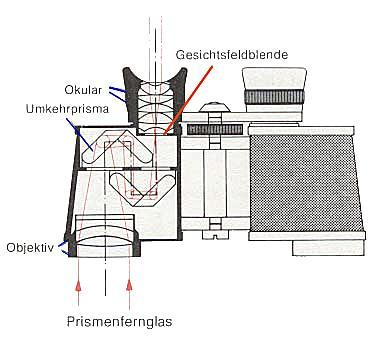
\includegraphics[width=0.49\textwidth]{gesichtsfledblende}}
% \caption{Gesichtsfeldblende und Umkehrprismen}
 \subfigure[Aperturblende]{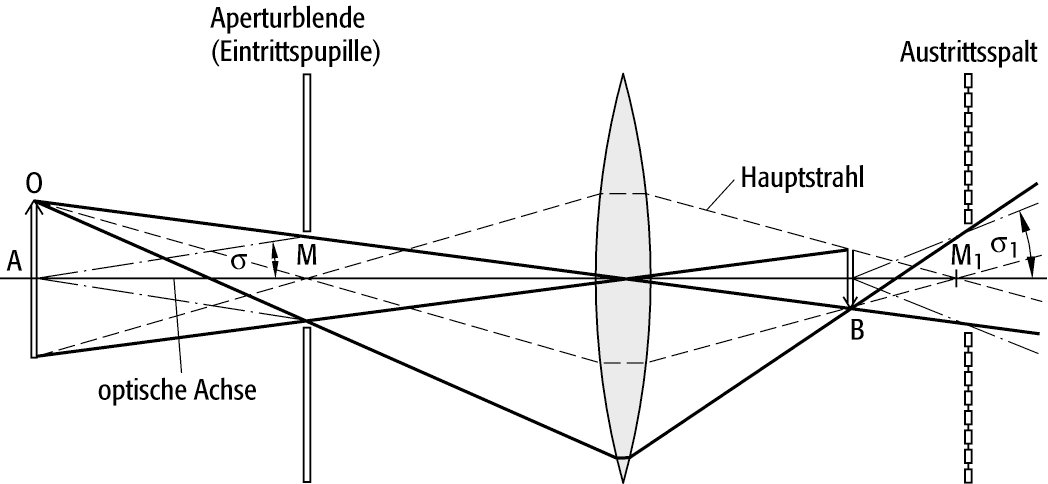
\includegraphics[width=0.49\textwidth]{Apertur}}
\end{figure}

7. Wie lassen sich in optischen Systemen mit einem vorgegebenen Linsensatz kurze Brennweiten
erzielen?\\
Es gilt: $\frac{1}{f}=\frac{1}{f_1}+\frac{1}{f_2}-\frac{d}{f_1f_2}$\\
$\rightarrow$ Kurze Brennweiten lassen sich durch einen möglichst kleinen Abstand d erzielen\\
\\8. Welche Linsenfehler gibt es? Nennen Sie Möglichkeiten zu ihrer Beseitigung!\\
\underline{sphärische Aberration:} bewirkt Unschärfe des Bildes; Beseitigung durch Unterdrückung achsenferner Strahlen mithilfe einer Blende\\
\underline{Astigmatismus:} Objekte, die außerhalb der optischen Achse liegen, werden unscharf abgebildet; Korrektur durch Kombination von sphärischen und torischen Gläsern. Die Hornhautverkrümmung kann auch operativ behandelt werden.\\
\\9. Erläutern Sie, warum Präzisionsfernrohre für die Astronomie nicht mit Linsen sondern mit
Spiegeln gebaut werden.\\
Es werden Spiegel benutzt, da sie eine größere Fläche abbilden können und billiger sind. Außerdem kann es keinen Farbfehler geben.\\\\
10. Zeichnen und erläutern Sie die Optik im menschlichen Auge! Erörtern Sie Kurz- und Weitsichtigkeit sowie Astigmatismus.\\
\begin{figure}[h]
 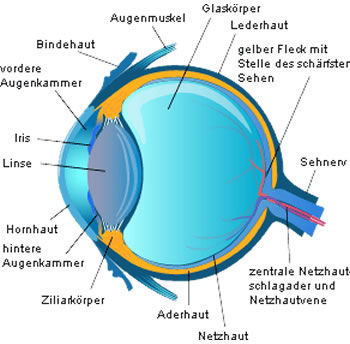
\includegraphics[width=0.5\textwidth]{Auge}
 \caption{Anatomie des Auges}
\end{figure}
Hornhaut: schützt das Auge nach außen\\
Iris und Pupille: Iris regelt Größe der Pupille und damit die Menge des durch die Linse durchtretenden Lichts\\
Linse: wesentliches Abbildungssystem des Auges\\
Glaskörper: Bestandteil des Abbildungssystems, sorgt für konst. Abstand Linse + Netzhaut\\
Netzhaut: beinhaltet Sehsinneszellen (Zäpfchen + Stäbchen)\\
Aderhaut: enthält Versorgungssystem für Netzhaut\\
Lederhaut: schützt das Auge nach außen
\underline{Kurzsichtigkeit:} zu langer Augapfel, der Fokus liegt vor der Netzhaut\\
\underline{Weitsichtigkeit:} zu kurzer Augapfel, der Fokus liegt hinter der Netzhaut\\
\underline{Astigmatismus:} siehe Aufgabe 8, Ursache: Hornhaut nicht exakt kreisförmig, sondern torisch, unterschiedliche Brechkraft an unterschiedlichen Stellen der Hornhaut, Strahlen bündeln sich nicht an einem Punkt
\\\\
11. Warum besteht der Kondensor eines Diaprojektors aus zwei plankonvexen Linsen? (Hinweis:
Berücksichtigen Sie die Reflexionsverluste!)
Plankonvexe Linsen werden benutzt, um die Dias besser auszuleuchten, ein möglichst großer Teil des Lichts der Projektionslampe soll in den abbildenden Strahlengang eingebracht werden, Verringerung der sphärischen Aberration und Totalreflexion\\
\\12. Wie kann man die Vergrößerung eines Fernrohrs ohne Kenntnis der Brennweiten messen?\\
Die Vergrößerung eines Fernrohres kann man mithilfe der Durchmesser ein- und ausfallenden Strahlenbündel bestimmen.\\
$V=\frac{d_{Aus}}{d_{Ein}}$ \\
\\13. Schätzen Sie die Größenordnung der Objektivbrennweite für einen Heimdiaprojektor ab, wenn Sie Raumgröße, Dia- und Leinwandgröße in Betracht ziehen\\
Leinwandgröße: 5m, Diagröße 5cm, Abstand zwischen linse und Dia: 10cm, Abstand zwischen LInse und Wand: 10m
Für Lupe gilt: $V=\frac{B}{G} \approx\frac{5m}{5cm}=100$ \\
Für Brennweite gilt: $f=(\frac{1}{0.1m}+\frac{1}{10m})^{-1}=9.9cm$
\\
\section{Durchführung}
\subsection{Lupe}
Betrachten Sie Gegenstände mit und ohne Lupe. Bestimmen Sie bei den verschiedenen Beobach
tungsarten jeweils die subjektiv ermittelten Vergrößerungen an.
\subsection{Astronomisches Fernrohr}
Material: 2 Achromate f = 500 mm, 60 mm und f = 40 mm, 10 mm Bikonvexlinse f = 500 mm, 38
mm 2 Bikonvexlinsen f = 40 mm, = 24 mm 2 Iris-Blenden, Ständer mit Schiene und Reiter
\begin{enumerate}
 \item   Bauen Sie ein astronomisches Fernrohr von mehr als 10-facher Vergrösserung aus zwei Bikon
 vexlinsen.
 \item Benutzen Sie eine Gesichtsfeldblende. Wo muss sie stehen, damit eine Gesichtsfeldbegrenzung
 bei Betrachtung sehr weit entfernter Gegenstände entsteht?
 \item  Benutzen Sie als Objektivlinse eine achromatische Linse. Beschreiben Sie die Unterschiede in
 der Bildgüte und bestimmen Sie die Vergrösserung experimentell.
 \item Stellen Sie eine Blende vor die Objektivlinse und betrachten Sie das Bild mit verschiedenen
 Durchmessern der Blende vor dem Objektiv
 \item Benutzen Sie als Okularlinse einen Achromaten
\end{enumerate}
\subsection{Terrestrisches Fernrohr}
Bauen Sie ein terrestrisches Fernrohr gem. Abb. og.3 auf. Diskutieren Sie insbesondere die Rolle
der mittleren Linse und ihren Einfluss auf die Vergrösserung. Untersuchen Sie die Eiflusse von
Linsenqualität (Achromate) und Blenden wie beim Astronomischen Fernrohr
\subsection{Holländisches Fernrohr}
Material: Achromat f = 500 mm, Bikonkavlinse f = -100 mm Bikonkavlinse f = -200 mm, Blende,
Ständer mit Schiene und Reitern
\begin{enumerate}
 \item . Welchen Eifluss hat der Objektivdurchmesser auf den Gesichtsfelddurchmesser?
 \item Bestimmen Sie den Durchmesser des Gesichtsfeldes bei 5-facher Vergrösserung und bei 2,5
 facher Vergrösserung (in beiden Fällen gleicher Objektivdurchmesser von 32 mm). Welcher Zu
 sammenhang besteht zwischen dem Durchmesser des Gesichtsfeldes und der Vergrösserung?
 \item Bestimmen Sie in beiden Fällen die Vergrösserung experimentell.
 
\end{enumerate}
\subsection{Spiegelteleskop}
Beobachten Sie weit entfernte Gegenstände mit dem Spiegelteleskop. Beurteilen Sie Vor- und Nach
teile gegenüber den vorher gebauten Fernrohren.
\subsection{Diaprojektor}
Vorhandene Komponenten: Bikonvexlinse f = 80 mm Optische Bank Achromat f = 80 mm Lampe
Kondensor f = 130 mm Diahalter mit Diapositiv Iris-Blende Schirm
Erzeugen Sie ein vergrößertes Bild des Diapositivs auf dem Schirm.
\begin{enumerate}
 \item  Beginnen Sie ohne Kondensorlinse mit einer Bikonvexlinse als Objektiv. Bilden Sie zunächst
 möglichst scharf ab bei einer Bildgrösse von ca. 10 cm. Verschieben Sie jetzt den Schirm so,
 dass das Bild etwas unscharf wird und verkleinern Sie dann mit der Irisblende den Linsen
 durchmesser. Beschreiben Sie die beobachteten Effekte.
 \item Benutzen Sie nun bei voller Objektivöffnung den Kondensor zur Beleuchtung des Diapositives
 und beschreiben Sie die Veränderungen im Bild gegenüber Aufgabe 1.
 \item Ändern Sie wieder wie in Aufgabe 1 den Objektivdurchmesser. Beschreiben Sie die beobach
 teten Effekte.
 \item Benutzen Sie nun als Objektiv eine korrigierte Linse (Achromat) mit gleicher Brennweite unter
 Konstanthalten der Abstände. Diskutieren Sie die Bildfehler (Farbfehler, Verzerrungen, fehlen
 de Schärfentiefe).
 
\end{enumerate}
\subsection{Mikroskop}
Geräte: Lampe (mit Kondensor), Dia mit Strichgitter d = 0,1 mm halbdurchlässiger Spiegel mit Halterung, Beobachtungsschirm Okular f = 25 mm (V = 10 ), Objektiv f = 40 mm, 10 mm Berechnen Sie die optischen Parameter eines Mikroskops für die Vergrösserung V = 50. Bestimmen Sie die Vergrösserung experimentell mit Hilfe der modifizierten Mikroskopanordnung in Abb.10: Nach der Okularlinse wird eine Sammellinse L (fL = 100 mm) platziert. Ein Beobachtungsschirm S wird im Abstand der Brennweite fL aufgestellt. Durch die Wirkung dieser Sammellinse werden die parallelen Lichtbündel, die die Okularlinse unter
dem Winkel $\psi$ verlassen auf einen Punkt am Beobachtungsschirm fokussiert. Die Vergrösserung V
des Mikroskopes kann bestimmt werden aus dem Verhältnis des Winkels $\psi$
und dem Winkel, unter
dem der Gegenstand G dem ünbewaffneten Augeïm Abstand der deutlichen Sehweite, s erscheint:
\begin{center}
 $V=\frac{\psi}{arctan g/s}$
\end{center}
Als Objekt benutzen Sie am besten das Strichgitter. Um den Winkelabstand zweier Gitterlinien auf
dem Schirm zu messen, bestimmen Sie die Höhe b, die von mehreren Gitterstrichen auf dem Beob
achtungsschirm eingenommen wird, und dividieren sie durch die Zahl der Zwischenräume zwischen
den betrachteten Gitterstrichen.


\end{document}